The GERDA (GERmanium Detector Array) experiment~\cite{Sch05} is designed to search for $0\nu\beta\beta$ decay of $^{76}$Ge. The main design feature is to operate naked germanium detectors directly in liquid argon in order to achieve extremely low background level. The concept is based on ideas presented in Ref~\cite{Heu95}. Detailed introduction of the experiment can be found in the first section of this chapter. GERDA is currently under construction in Hall A of the INFN Gran Sasso National Laboratory (LNGS), Italy. The current status of the experiment is described in the second section. The development of GERDA is divided into three phases. In the first phase (Phase I) unsegmented germanium detectors, which were previously used in IGEX~\cite{Aal02} and HdM~\cite{Hei04} experiments, will be re-deployed. The envisioned background level is $10^{-2}$~events/(kg$\cdot$keV$\cdot$year). In the second phase (Phase II) 18-fold segmented detectors, which currently are under construction, will be used in addition. The aimed background level is $10^{-3}$~events/(kg$\cdot$keV$\cdot$year). A later phase (Phase III) is under discussion in cooperation with the MAJORANA Collaboration~\cite{Gai03,Aal04} aiming at a one tonne scale experiment. The physics observation capabilities of three phases of GERDA are discussed in the last section.

\section{Concept}
\label{sec:gerda:conc}
The germanium detector has been used to detect ionizing radiation, particularly X-rays and $\gamma$-rays for years. It has energy resolution better than 1\% around the $Q$-value region of the $0\nu\beta\beta$ decay, which is among the bests in all $0\nu\beta\beta$ decay detectors introduced in Sec.~\ref{sec:gencon}. This provides very good separation of $0\nu\beta\beta$ decay signal from $2\nu\beta\beta$ decay background. However, the natural abundance of $^{76}$Ge (7.6\%) is not very high, hence additional enrichment is needed. And the $Q$-value of the $0\nu\beta\beta$ decay of $^{76}$Ge, 2.039~MeV, is still lower than some of the natural radiation lines. Special designs are needed to reduce the background. Fig.~\ref{fig:gerda} shows the engineering drawing of the structure of GERDA. Each part of the structure is introduced in the following sections as well as its functionality of reducing background from different sources.

\begin{figure}[tbhp]
  \centering
  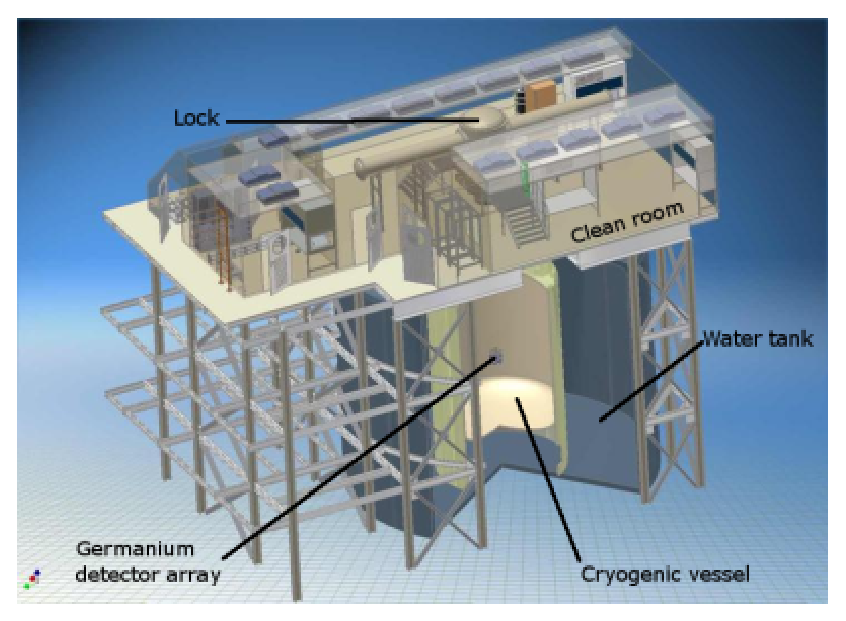
\includegraphics[width=0.7\textwidth]{gerda}  
  \caption{Structure of GERDA from engineer's view.}
  \label{fig:gerda}
\end{figure}

\subsection{Location and muon veto}
\label{sec:gerda:loca}
In order to reduce the cosmic ray induced background GERDA was chosen to be located in Hall A of the INFN Gran Sasso National Laboratory (LNGS), Italy. LNGS is the largest underground facility in the world for low-background experiments. It can be accessed from a 10~km long highway tunnel under the Gran Sasso mountains. It has three experimental halls hosting a large variety of experiments, most of which focus on dark matter or neutrino physics. Fig.~\ref{fig:lngs} shows the location of GERDA in LNGS. The main experimental site of GERDA is between the Large Volume Detector (LVD) and a service tunnel across Hall A. The GERDA auxiliary and cryogenic storage system will be located in the service tunnel on the northeast side of Hall A.

\begin{figure}[tbhp]
  \centering
  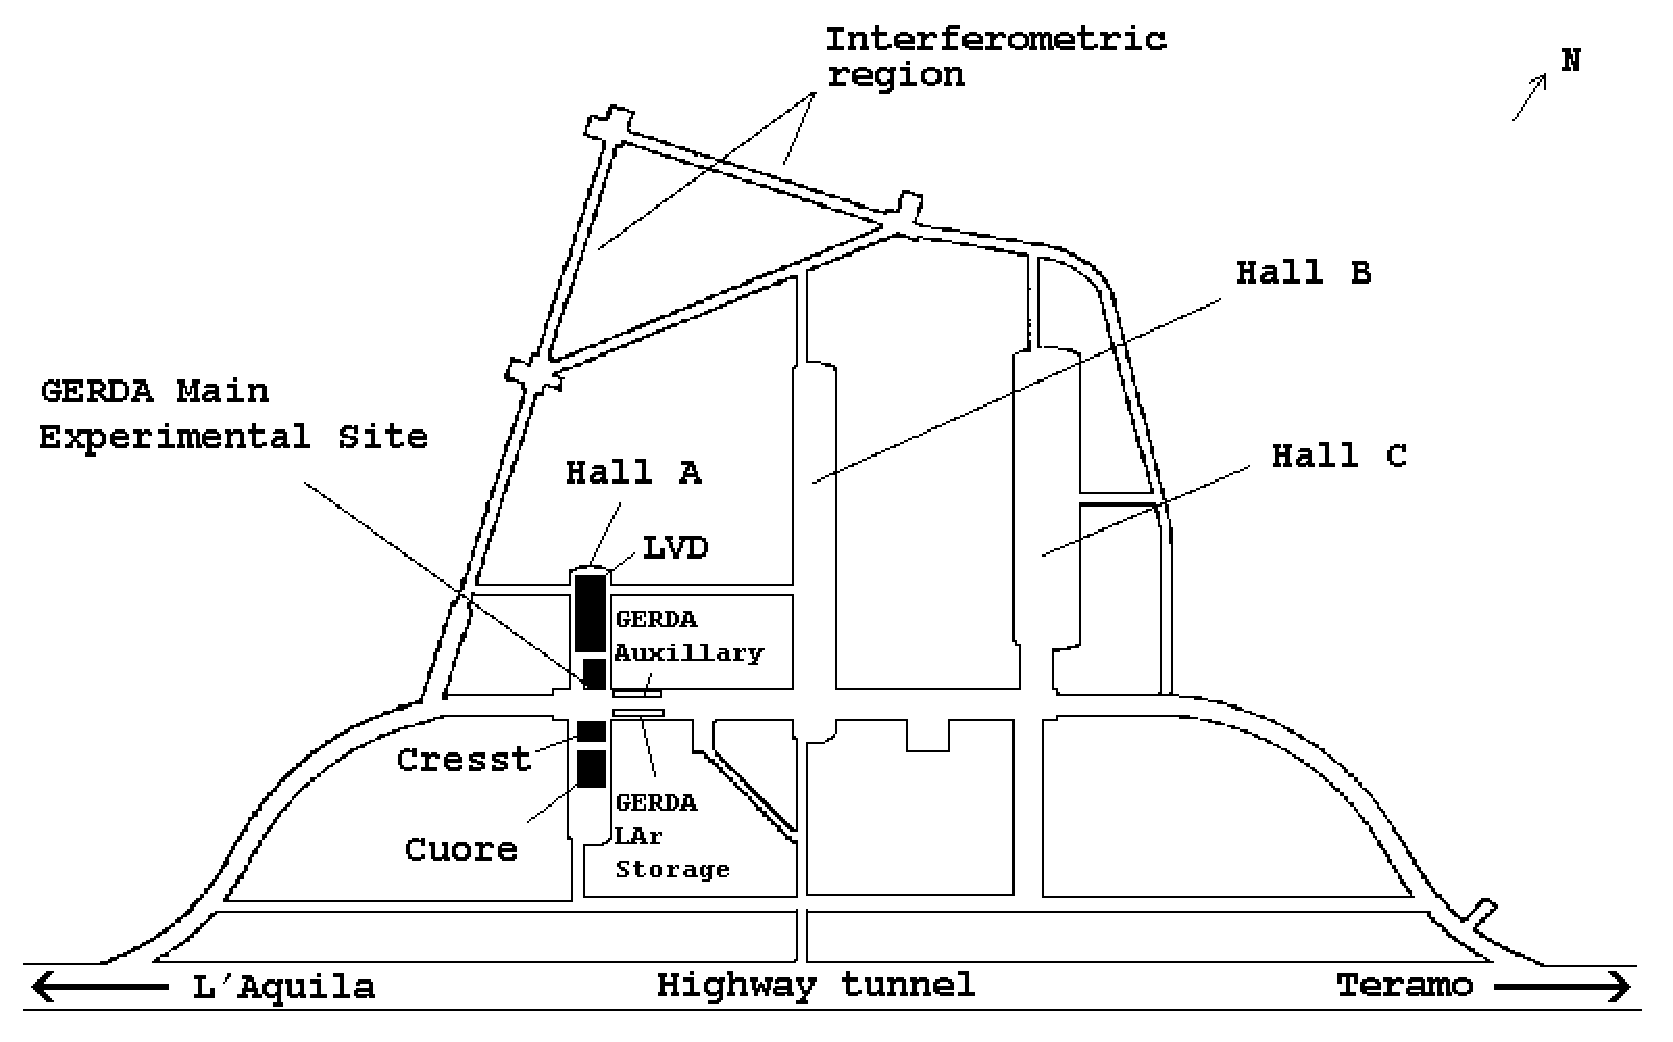
\includegraphics[width=0.8\textwidth]{lngs}  
  \caption{Location of GERDA in LNGS. The main experimental site of     GERDA is between the Large Volume Detector (LVD) and a service     tunnel across Hall A. The GERDA auxiliary and cryogenic storage     system will be located in the service tunnel on the northeast side     of Hall A.}
  \label{fig:lngs}
\end{figure}

The overburden of 1.4~km of rock on top of the experimental halls corresponds to 3.4~km meter of water equivalent (m.w.e). It reduces the cosmic ray induced muon flux by a factor of $10^{6}$, and neutron flux a factor of $10^{3}$ compared to the surface. The energy and angular distribution of cosmic ray muons in Hall A of LNGS have been precisely measured~\cite{Amb95, Lip91, Amb03}. A comprehensive study of cosmic ray induced muon and neutron background in underground laboratories can be found in Ref.~\cite{Mei06}.

In order to further reduce the muon induced background additional muon veto system will be implemented. Cosmic muons traversing the water buffer will cause Cherenkov radiation. To detect the radiation 66 photomultiplier tubes (PMTs) will be installed on the walls of the water tank. The positions of PMTs are optimized according to Monte Carlo simulation. Together with these PMTs the water tank could be operated as a Cherenkov detector. The detection efficiency is about 95\% depending on the incident angle of the muon. In order to compensate for the missing water volume around the neck of the cryostat plastic scintillator plates will be placed on top of the clean room. They are used to detect the muons entering the cryostat almost vertically. The combined detection efficiency is expected to be above 99\%.

\subsection{Water tank and cryostat}
\label{sec:gerda:rock}
To mediate and absorb the neutron radiation from the rock $\sim 630$~m$^{3}$ of ultra-pure water will be filled in a stainless steel tank with an outer diameter of 10~m and a height of about 8~m. Since liquid argon can be produced with a much greater purity than lead or even copper traditionally used for shielding, a total of approximately 98~t of liquid argon will be stored in a cryostat placed inside the water tank to shield $\gamma$-rays from the rock and water. The vessel is made of stainless steel with an internal copper liner. The height of the vessel is 5.88~m (7.62~m with the neck) while the outer diameter is 4.16~m.

\subsection{Detector suspension system and electronics}
\label{sec:gerda:cable}
Germanium detectors will be suspended in liquid argon from the top of the cryostat. In order to minimize the contamination from the suspension system, signal and high voltage cables light-weighted detector holding frames and novel contacting scheme shown in the left plot of Fig.~\ref{fig:array} will be used. The frames are made of thin ultra-pure copper bars with a total weight of about 30~g. They will be chained vertically into strings. Each string consists of 3 detectors with the same type, as shown in the middle plot of Fig.~\ref{fig:array}. The whole detector array could maximally consists of 16 hexagonally packed detector strings as shown in the right plots of Fig.~\ref{fig:array}. 

The horizontal distance between the centers of two detectors is 9~cm. The vertical clearance between two detectors is about 6~cm. The Phase I detectors are p-type diodes with a cylindrical closed-ended coaxial geometry. The detectors are enriched in $^{76}$Ge to a level of about 86\% and have masses between 0.9~kg and 2.9~kg. The detectors for Phase II will be cylindrical true coaxial n-type diodes. The precise size of the detectors will depend on manufacturing details. The most likely dimensions are a height of 70~mm and a diameter of 75~mm. The detectors will be segmented. The segmentation scheme under consideration is a 6-fold segmentation in the azimuthal angle $\phi$ and a 3-fold segmentation in the height z. 

\begin{figure}[tbhp]
  \centering
  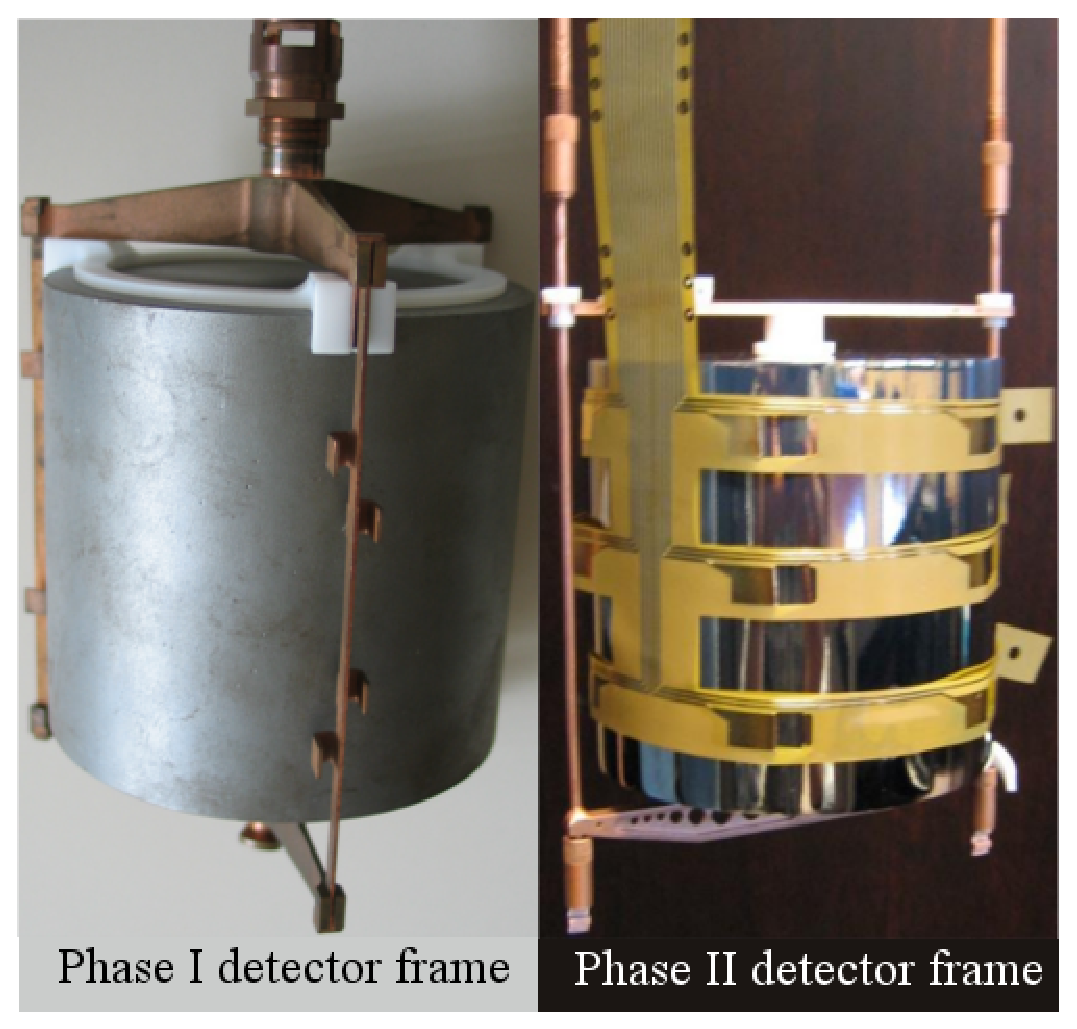
\includegraphics[width=0.33\textwidth]{detectorFrame}
  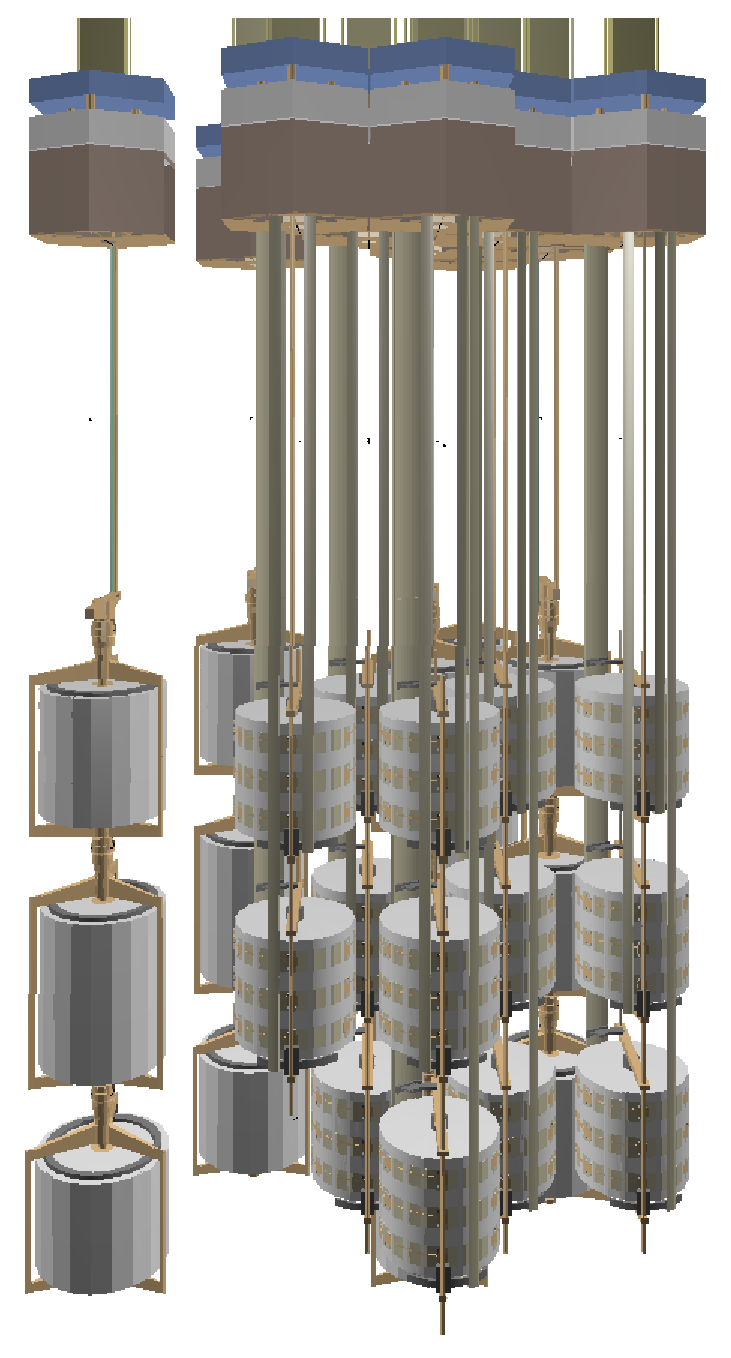
\includegraphics[width=0.2\textwidth]{array}   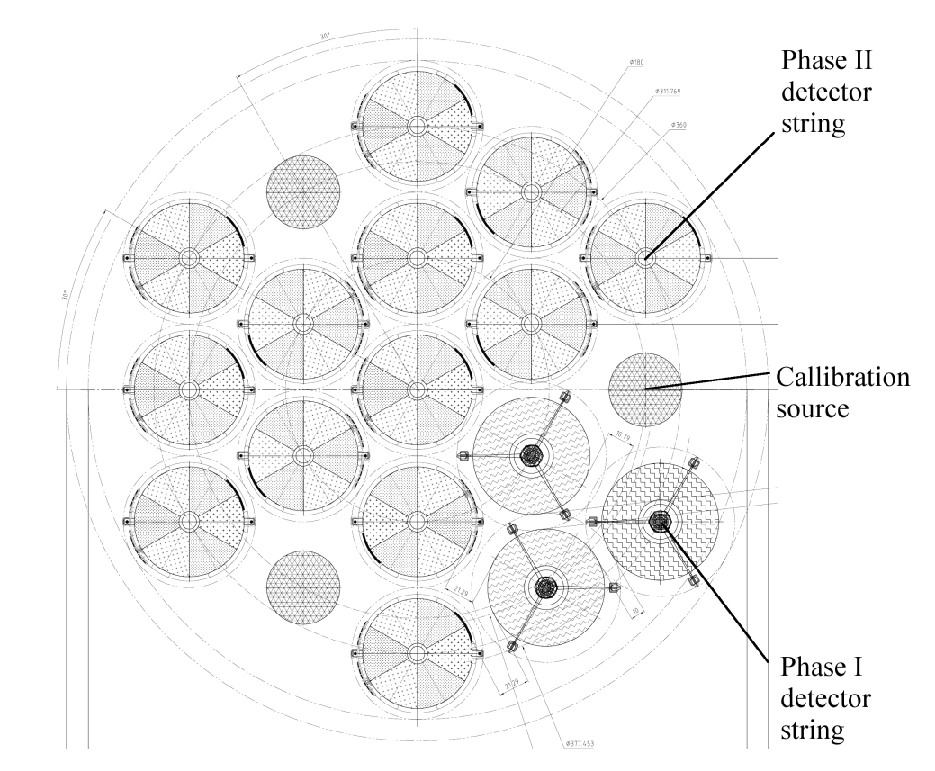
\includegraphics[width=0.45\textwidth]{arrayTop}
  \caption{Detector array configuration. The left plot shows single     Phase I detector with copper frame and Phase II detector with     copper frame and a novel contacting scheme. The middle plot shows     how the detectors are chained into strings and hung together in     liquid argon.  The right plot shows the top view of the full array     indicating the possible positions for the Phase I and Phase II     detector strings as well as for the calibration sources.}
  \label{fig:array}
\end{figure}

A couple of solutions are actively pursued for the read-out electronics of GERDA~\cite{Cat07}. A common scheme foresees a cold FET close to the crystal followed by amplifying and load driving circuits located at room temperature. The cold FET would be placed near the connection matrix (top blocks in the middle plot of Fig.~\ref{fig:array}) 30~cm above the detector array. Pre-amplified signals would be sent to circuits at room temperature through 6~m long cables, as this is the minimum distance from crystal to room temperature environment.

\subsection{Detector storage and clean room}
\label{sec:gerda:source}
When processed or transfered above ground, germanium detectors are exposed to cosmic radiation and radioactive isotopes could be produced inside the detector through spallation caused by energetic cosmic rays. Two cosmogenic isotopes, $^{60}$Co and $^{68}$Ge, have Q-values above that of $^{76}$Ge $0\nu\beta\beta$ decay and are potential sources of background. Therefore the detector processing time above ground needs to be minimized. Since the half life time of $^{60}$Co and $^{68}$Ge is 5.3 years and 271 days, respectively, a passive method to reduce their contamination is to wait long enough so that most of them decay.

When exposed to the air, germanium detector surface may be contaminated by dust which contains many radioactive isotopes undergoing $\alpha$ decay. The detector surface is not fully charge sensitive and only part of the energy lost by the $\alpha$ particle can be detected. This may result in a signal close to the $Q$-value of $^{76}$Ge $0\nu\beta\beta$ decay. Therefore the testing, preparation and insertion of the detector need to be done in a rather clean environment. For this purpose, a class 10000 clean room with radon-reduced air will be built on top of the cryostat. It houses a lock through which detector strings are inserted into and removed from the cryogenic volume. Detector handling will be performed in flow-boxes and a detector mounting station which will reach class 100.  The lock consists of a rail system which allows to move detector strings into their correct position and lower them into the cryostat. In addition, the clean room will be used to temporarily store germanium detectors under a controlled atmosphere of gaseous argon as shown in Fig.~\ref{fig:store}.

\begin{figure}[tbhp]
  \centering
  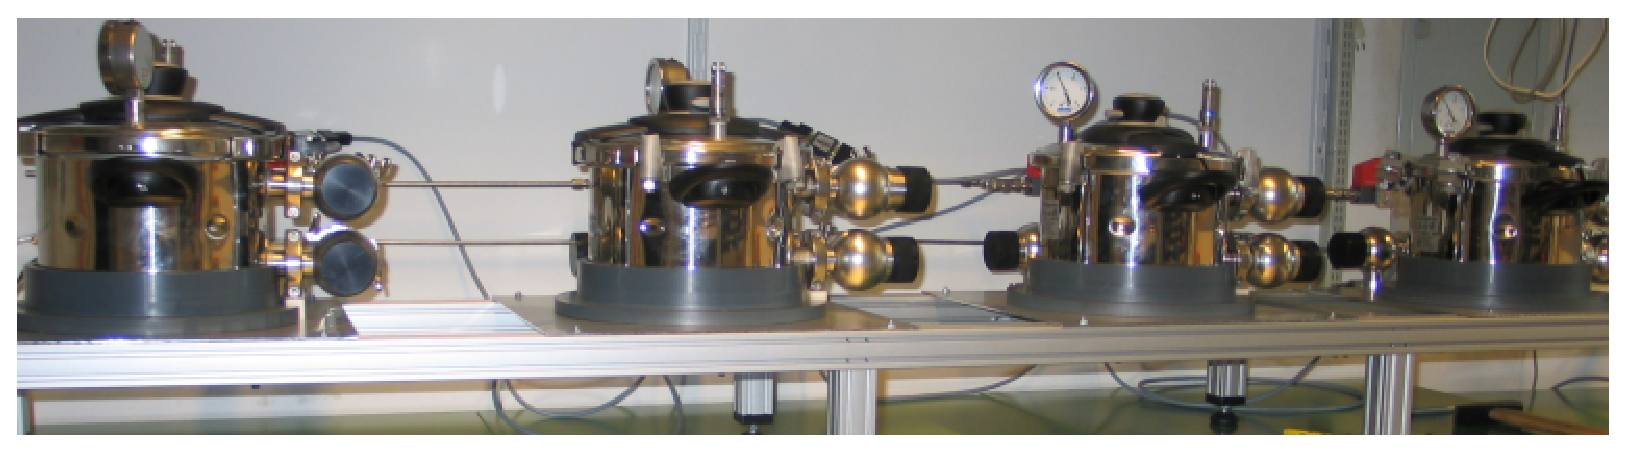
\includegraphics[width=\textwidth]{storage}
  \caption{Detector storage system. The left plot shows an open vacuum     can with a detector inside. The middle plot shows a closed vacuum     can equipped with valves and gas flux sensor. The right plot shows     four vacuum cans connected with gas tubes.}
  \label{fig:store}
\end{figure}

\subsection{Other background rejection techniques}
\label{sec:gerda:anti}
Other background rejection techniques that can be used in GERDA include 1. anti-coincidence measurement, 2. pulse shape analysis, and 3. instrumentation of the cryostat.
\begin{description}
\item[Anti-coincidence] Compton-scattered photons are likely to   deposit energy in more than one detector while $0\nu\beta\beta$   decay electrons will predominantly deposit energy in only one   detector. Photons can thus be identified by requiring more than one   detector to see energy above the threshold. Considering the   segmented detectors for Phase II photons depositing energy in one   crystal can still be identified by requiring more than one segment   to show energy. Time anti-coincidence veto could also be used to   reject background induced by the decay of $^{68}$Ge and $^{77}$Ge   meta stable state. Feasibility studies are currently carried out.
\item[Pulse shape analysis] Although photons are likely to create more   than one energy deposition, if these energy depositions are confined   to one segment, the anti-coincidence between segments cannot   distinguish this kind of event from $0\nu\beta\beta$ decay signal.   However, by analyzing the time structure of the detector response,   \textit{i.e.} pulse shape, photons and electrons can be further   distinguished~\cite{Kev07}.
\item[instrumentation of the cryostat] Liquid argon scintillates if   energy is deposited inside the argon volume. The scintillation light   can be detected by PMT's mounted on the walls of the cryostat.   Events with photons in the final state which deposit only a fraction   of their energy inside the germanium detectors can be vetoed by   requiring an anti-coincidence between the observed scintillation   light and the energy deposit inside the detectors.  This technique   is not part of the GERDA baseline design. Feasibility studies are   currently being performed~\cite{Pei05, Orr06}.
\end{description}

\section{Status}
\label{sec:gerda:stat}
This section closes with the status of GERDA as of Winter 2008/09. Important milestones and results are summarized below.  

\subsection{Cryostat and water tank}
\label{sec:gerda:stat1}
On 6 March 2008, the cryostat was delivered to LNGS and placed at the foreseen location in Hall A, as shown in the middle plot of Fig.~\ref{fig:cryo}. Mounting of the internal copper shield was completed on March 18. The cryostat passed several acceptance tests including pressure tests, helium leak tests, liquid nitrogen evaporation tests and radon emanation measurements. The water tank installation finished at the end of June, as shown in the right plot of Fig.~\ref{fig:cryo}. The installation of the cryostat and water tank with the design specifications is a major milestone for GERDA.

\begin{figure}[tbhp]
  \centering
  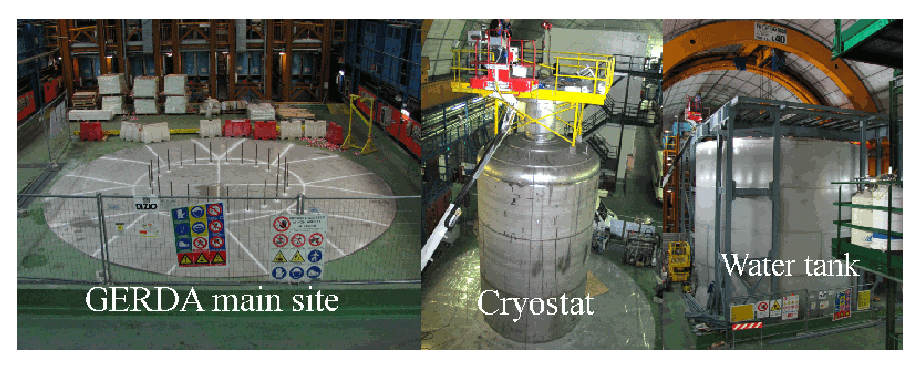
\includegraphics[width=\textwidth]{cryostat}
  \caption{Construction of cryostat and water tank in GERDA main site.     From left to right: the empty GERDA main site, the installed     cryostat and water tank and some infrastructure around it.}
  \label{fig:cryo}
\end{figure}

\subsection{Clean room and lock system}
\label{sec:gerda:stat2}
As shown in the right plot of Fig.~\ref{fig:cryo}, the construction of the infrastructure around the water tank is ongoing, on top of which the clean room and lock will be erected. The design of the clean room is finished. The construction is scheduled to finish at February 2009. The design of the complete lock structure is almost finished. The lock will be preinstalled at the Max-Planck-Institut f\"ur Physik in Munich and then transported to LNGS early 2009. A provisional lock system is in production. It will be used before the complete lock system is ready so that the commissioning of GERDA could start at February 2009.

\subsection{Phase I and II detectors}
\label{sec:gerda:stat3}
In total 17.9~kg of enriched and 15~kg of non-enriched high-purity p-type germanium detectors from IGEX, HdM and Genius Test Facility (GTF)~\cite{Kla02} will be operated in Phase I of GERDA.  Stability tests of the operation of p-type detectors in cryogenic liquids are practically completed.  After two years of operation with more than 50 warming and cooling cycles, the $\gamma$-ray induced leakage current has been proved to be negligible if the passivation layer is limited to the groove area only, and the detector handling procedure has been defined.

In total 14 segmented germanium detector, each weighs 1.62~kg, will be used for GERDA Phase II. 37.5~kg enriched germanium dioxide, which will be used to produce Phase II detectors is stored in the HADES underground facility. The yield for the purification of GeO$_{2}$ to 6N metal is about 90\% and the time above ground for the purification will not exceed 2 to 3 days. The crystal will be grown in the Institut f\"ur Kristallz\"uchtung (IKZ) in Berlin. Small crystals from zone-refined material with the concentration of impurities between $10^{12}$ and $10^{11}$ per cm$^{3}$ has been pulled in IKZ, as shown in Fig.~\ref{fig:pulling}. The Czochralski puller has been refurbished already set up to produce 2~inch crystals.
\begin{figure}[tbhp]
  \centering
  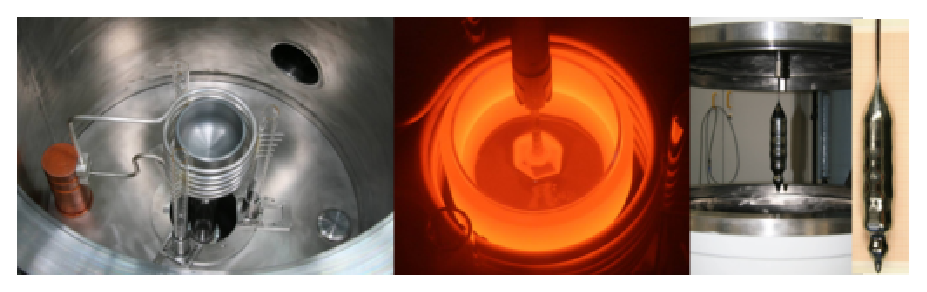
\includegraphics[width=\textwidth]{crystalPulling}
  \caption{Pulling crystal in Czochralski puller. From left to right: Czochralski puller, pulling crystal, pulled crystal and a close look of it.}
  \label{fig:pulling}
\end{figure}

The first Phase II prototype detector operated in a conventional cryostat has been tested and characterized~\cite{Sie07}. The second prototype detector has been equipped with the novel signal contacts and operated in liquid nitrogen for months. The handling, operating and testing of the prototype detectors and the physics analysis based on the data from them are the main topics of this thesis and will be discussed in detail in the following chapters.


\subsection{Other progress}
\label{sec:gerda:stat4}
Front-End electronics has been tested in liquid nitrogen with two new detector test stands, namely, Sub with a p-type detector and Gerdella with an n-type detector. Measurements with Sub gave an energy resolution of 2.6~keV (FWHM) at 1.3~MeV. Optimization in terms of noise performance is ongoing and further improvements expected.

As for muon veto system, a batch of 10 plastic scintillator panels has been assembled at Dubna and tested in LNGS. The tests have shown that the concept works. And the PMT production has successfully completed. 

The behavior of radon and its daughters in liquid nitrogen has been studied. It has been proved that radon would not be taken away by boiled-off nitrogen and stays predominantly in the liquid, and that radon, in particular its progenies $^{214}$Po and $^{218}$Po are attracted to steel plates if either positive or negative high voltage is applied. Measurements in argon and with germanium substrates are now under preparation. This effect, if it persists in LAr/Ge, would offer the possibility to remove actively residual radon traces by implementing electrodes to sweep out radon and their progenies. 


\section{Sensitivity}
\label{sec:gerda:sens}
A dedicated discussion about the sensitivity of GERDA can be found
in Ref.~\cite{Cal06}. The left plot in Fig.~\ref{fig:gerda:limit}
taken from Ref.~\cite{Cal06} shows the expected 90\% probability lower
limit on the half lifetime for $0\nu\beta\beta$ decay versus the
exposure under different background conditions. Also shown is the half
lifetime for the claimed observation by H. V. Klapdor-Kleingrothaus
\textit{et al.}~\cite{Hei04}. The right plot shows the expected 90\%
probability upper limit on the effective Majorana neutrino mass versus
the exposure under different background conditions. The effective
Majorana neutrino mass for the claimed observation is also shown. All
mass values are determined from the half lifetime using the matrix
element reported in Ref~\cite{Rod07}.
\begin{figure}[tbhp]
  \centering
  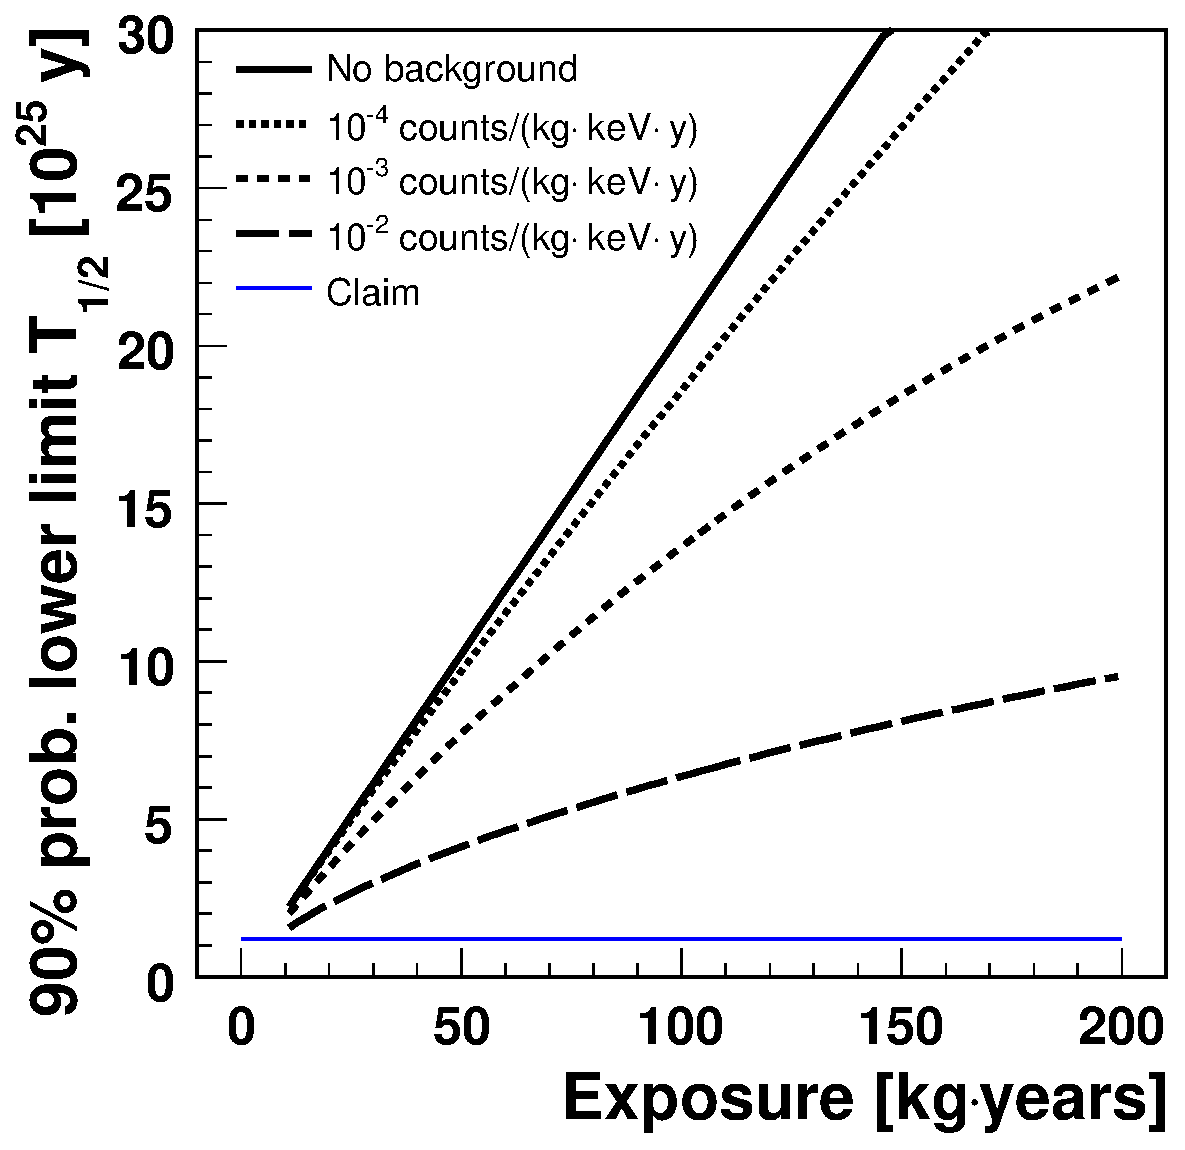
\includegraphics[width=0.45\textwidth]{limit_halflife}  \hfil
  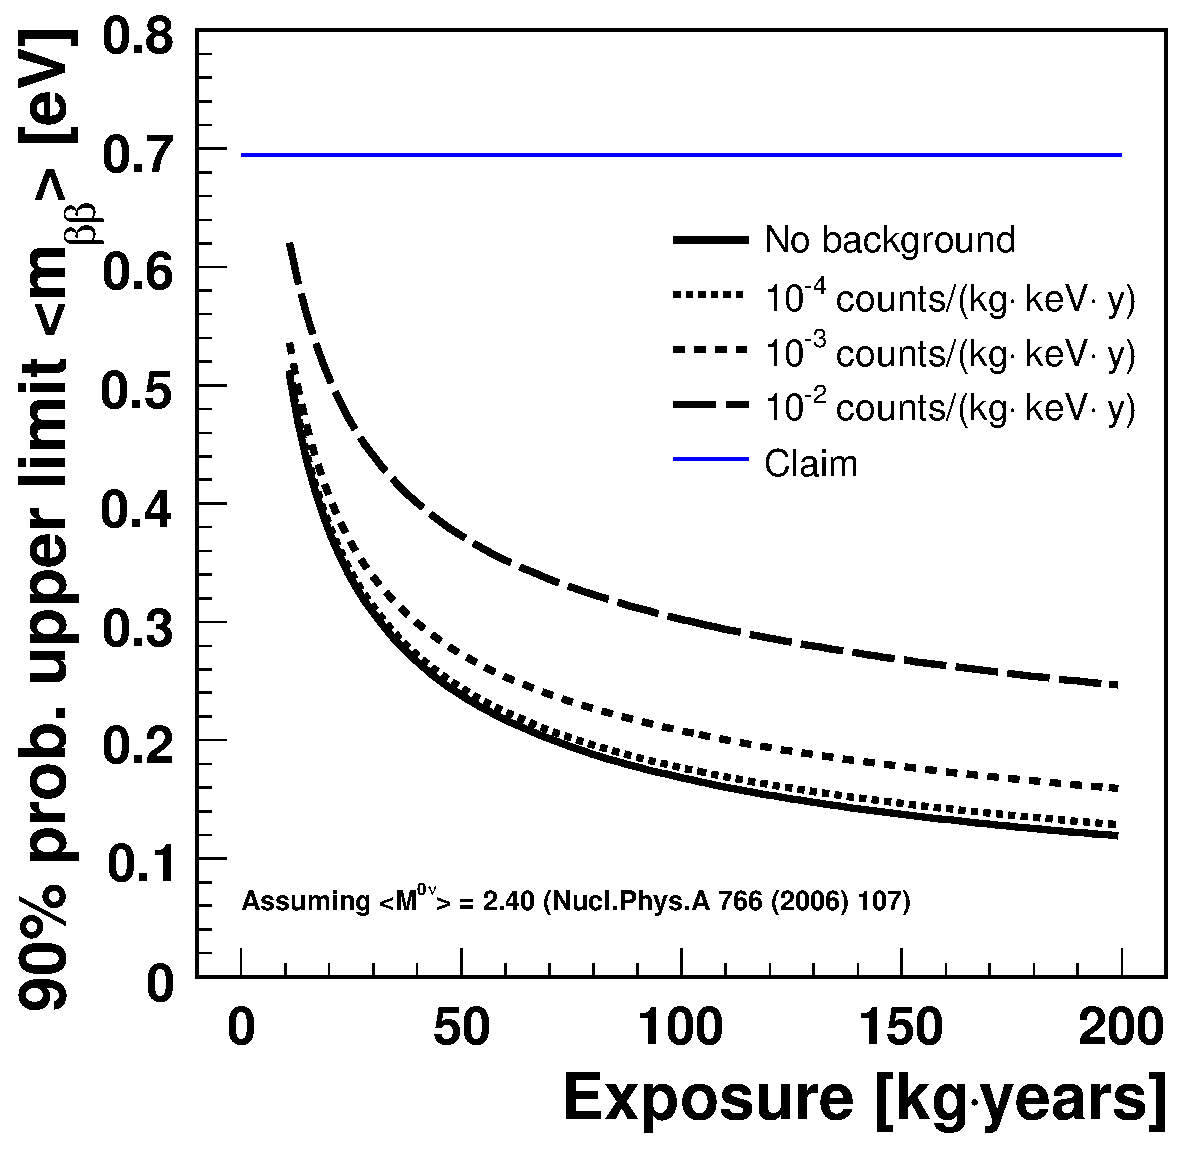
\includegraphics[width=0.45\textwidth]{limit_mass}
  \caption{The expected 90\% probability lower limit on the half    
lifetime for $0\nu\beta\beta$ decay (left) and the expected 90\%    
probability upper limit on the effective Majorana neutrino mass    
(right) versus the exposure under different background conditions.    
Also shown is the half lifetime and the effective Majorana    
neutrino mass for the claimed observation by H. V.    
Klapdor-Kleingrothaus \textit{et al.}~\cite{Hei04}. All mass    
values are determined from the half lifetime using the matrix    
element reported in Ref~\cite{Rod07}.}
  \label{fig:gerda:limit}
\end{figure}

For GERDA Phase I, assuming a background level of $10^{-2}$~events/(kg$\cdot$keV$\cdot$year) and an exposure of
100~(kg$\cdot$year), an upper limit on $m_{\beta\beta}$ of
0.3~eV would be achievable. For Phase II, assuming a background level of $10^{-3}$~events/(kg$\cdot$keV$\cdot$year) and an exposure of
100~(kg$\cdot$year), an upper limit on $m_{\beta\beta}$ of
0.2~eV would be achievable.


%%% Local Variables:
%%% mode:latex
%%% TeX-master: "thesis"
%%% End:
